% Options for packages loaded elsewhere
% Options for packages loaded elsewhere
\PassOptionsToPackage{unicode}{hyperref}
\PassOptionsToPackage{hyphens}{url}
\PassOptionsToPackage{dvipsnames,svgnames,x11names}{xcolor}
%
\documentclass[
  preprint, 3p, authoryear]{article}
\usepackage{xcolor}
\usepackage{amsmath,amssymb}
\setcounter{secnumdepth}{-\maxdimen} % remove section numbering
\usepackage{iftex}
\ifPDFTeX
  \usepackage[T1]{fontenc}
  \usepackage[utf8]{inputenc}
  \usepackage{textcomp} % provide euro and other symbols
\else % if luatex or xetex
  \usepackage{unicode-math} % this also loads fontspec
  \defaultfontfeatures{Scale=MatchLowercase}
  \defaultfontfeatures[\rmfamily]{Ligatures=TeX,Scale=1}
\fi
\usepackage{lmodern}
\ifPDFTeX\else
  % xetex/luatex font selection
\fi
% Use upquote if available, for straight quotes in verbatim environments
\IfFileExists{upquote.sty}{\usepackage{upquote}}{}
\IfFileExists{microtype.sty}{% use microtype if available
  \usepackage[]{microtype}
  \UseMicrotypeSet[protrusion]{basicmath} % disable protrusion for tt fonts
}{}
\makeatletter
\@ifundefined{KOMAClassName}{% if non-KOMA class
  \IfFileExists{parskip.sty}{%
    \usepackage{parskip}
  }{% else
    \setlength{\parindent}{0pt}
    \setlength{\parskip}{6pt plus 2pt minus 1pt}}
}{% if KOMA class
  \KOMAoptions{parskip=half}}
\makeatother
% Make \paragraph and \subparagraph free-standing
\makeatletter
\ifx\paragraph\undefined\else
  \let\oldparagraph\paragraph
  \renewcommand{\paragraph}{
    \@ifstar
      \xxxParagraphStar
      \xxxParagraphNoStar
  }
  \newcommand{\xxxParagraphStar}[1]{\oldparagraph*{#1}\mbox{}}
  \newcommand{\xxxParagraphNoStar}[1]{\oldparagraph{#1}\mbox{}}
\fi
\ifx\subparagraph\undefined\else
  \let\oldsubparagraph\subparagraph
  \renewcommand{\subparagraph}{
    \@ifstar
      \xxxSubParagraphStar
      \xxxSubParagraphNoStar
  }
  \newcommand{\xxxSubParagraphStar}[1]{\oldsubparagraph*{#1}\mbox{}}
  \newcommand{\xxxSubParagraphNoStar}[1]{\oldsubparagraph{#1}\mbox{}}
\fi
\makeatother


\usepackage{longtable,booktabs,array}
\usepackage{calc} % for calculating minipage widths
% Correct order of tables after \paragraph or \subparagraph
\usepackage{etoolbox}
\makeatletter
\patchcmd\longtable{\par}{\if@noskipsec\mbox{}\fi\par}{}{}
\makeatother
% Allow footnotes in longtable head/foot
\IfFileExists{footnotehyper.sty}{\usepackage{footnotehyper}}{\usepackage{footnote}}
\makesavenoteenv{longtable}
\usepackage{graphicx}
\makeatletter
\newsavebox\pandoc@box
\newcommand*\pandocbounded[1]{% scales image to fit in text height/width
  \sbox\pandoc@box{#1}%
  \Gscale@div\@tempa{\textheight}{\dimexpr\ht\pandoc@box+\dp\pandoc@box\relax}%
  \Gscale@div\@tempb{\linewidth}{\wd\pandoc@box}%
  \ifdim\@tempb\p@<\@tempa\p@\let\@tempa\@tempb\fi% select the smaller of both
  \ifdim\@tempa\p@<\p@\scalebox{\@tempa}{\usebox\pandoc@box}%
  \else\usebox{\pandoc@box}%
  \fi%
}
% Set default figure placement to htbp
\def\fps@figure{htbp}
\makeatother


% definitions for citeproc citations
\NewDocumentCommand\citeproctext{}{}
\NewDocumentCommand\citeproc{mm}{%
  \begingroup\def\citeproctext{#2}\cite{#1}\endgroup}
\makeatletter
 % allow citations to break across lines
 \let\@cite@ofmt\@firstofone
 % avoid brackets around text for \cite:
 \def\@biblabel#1{}
 \def\@cite#1#2{{#1\if@tempswa , #2\fi}}
\makeatother
\newlength{\cslhangindent}
\setlength{\cslhangindent}{1.5em}
\newlength{\csllabelwidth}
\setlength{\csllabelwidth}{3em}
\newenvironment{CSLReferences}[2] % #1 hanging-indent, #2 entry-spacing
 {\begin{list}{}{%
  \setlength{\itemindent}{0pt}
  \setlength{\leftmargin}{0pt}
  \setlength{\parsep}{0pt}
  % turn on hanging indent if param 1 is 1
  \ifodd #1
   \setlength{\leftmargin}{\cslhangindent}
   \setlength{\itemindent}{-1\cslhangindent}
  \fi
  % set entry spacing
  \setlength{\itemsep}{#2\baselineskip}}}
 {\end{list}}
\usepackage{calc}
\newcommand{\CSLBlock}[1]{\hfill\break\parbox[t]{\linewidth}{\strut\ignorespaces#1\strut}}
\newcommand{\CSLLeftMargin}[1]{\parbox[t]{\csllabelwidth}{\strut#1\strut}}
\newcommand{\CSLRightInline}[1]{\parbox[t]{\linewidth - \csllabelwidth}{\strut#1\strut}}
\newcommand{\CSLIndent}[1]{\hspace{\cslhangindent}#1}



\setlength{\emergencystretch}{3em} % prevent overfull lines

\providecommand{\tightlist}{%
  \setlength{\itemsep}{0pt}\setlength{\parskip}{0pt}}



 


\usepackage[noblocks]{authblk}
\renewcommand*{\Authsep}{, }
\renewcommand*{\Authand}{, }
\renewcommand*{\Authands}{, }
\renewcommand\Affilfont{\small}
\usepackage{xcolor}
\usepackage{lscape}
\newcommand{\blandscape}{\begin{landscape}}
\newcommand{\elandscape}{\end{landscape}}
\usepackage{geometry}
\geometry{
  top=2.5cm,
  bottom=2.5cm,
  left=2.5cm,
  right=2.5cm
}
\usepackage{pdflscape}
\usepackage{lineno}
\usepackage{threeparttable}
\makeatletter
\@ifpackageloaded{caption}{}{\usepackage{caption}}
\AtBeginDocument{%
\ifdefined\contentsname
  \renewcommand*\contentsname{Table of contents}
\else
  \newcommand\contentsname{Table of contents}
\fi
\ifdefined\listfigurename
  \renewcommand*\listfigurename{List of Figures}
\else
  \newcommand\listfigurename{List of Figures}
\fi
\ifdefined\listtablename
  \renewcommand*\listtablename{List of Tables}
\else
  \newcommand\listtablename{List of Tables}
\fi
\ifdefined\figurename
  \renewcommand*\figurename{Figure}
\else
  \newcommand\figurename{Figure}
\fi
\ifdefined\tablename
  \renewcommand*\tablename{Table}
\else
  \newcommand\tablename{Table}
\fi
}
\@ifpackageloaded{float}{}{\usepackage{float}}
\floatstyle{ruled}
\@ifundefined{c@chapter}{\newfloat{codelisting}{h}{lop}}{\newfloat{codelisting}{h}{lop}[chapter]}
\floatname{codelisting}{Listing}
\newcommand*\listoflistings{\listof{codelisting}{List of Listings}}
\makeatother
\makeatletter
\makeatother
\makeatletter
\@ifpackageloaded{caption}{}{\usepackage{caption}}
\@ifpackageloaded{subcaption}{}{\usepackage{subcaption}}
\makeatother
\usepackage{bookmark}
\IfFileExists{xurl.sty}{\usepackage{xurl}}{} % add URL line breaks if available
\urlstyle{same}
\hypersetup{
  pdftitle={Validating OpenStreetMap for detecting cycling-infrastructure change: A Barcelona pilot using Google Street View (2015--2023)},
  pdfauthor={Eugeni Vidal-Tortosa; Monika Maciejewska; Oriol Marquet},
  colorlinks=true,
  linkcolor={blue},
  filecolor={Maroon},
  citecolor={Blue},
  urlcolor={Blue},
  pdfcreator={LaTeX via pandoc}}


\title{Validating OpenStreetMap for detecting cycling-infrastructure
change: A Barcelona pilot using Google Street View (2015--2023)}


\author[1]{Eugeni Vidal-Tortosa}
\author[1]{Monika Maciejewska}
\author[1, 2]{Oriol Marquet}

\affil[1]{Department of Geography, Universitat Autònoma de Barcelona
(UAB), Bellaterra Campus, Building B, Carrer de la Fortuna, s/n, 08193,
Bellaterra, Barcelona, Spain}
\affil[2]{Institute of Environmental Science and Technology (ICTA-UAB),
Building ICTA-ICP, Carrer de les Columnes s/n, UAB Campus, 08193,
Cerdanyola del Vallès, Barcelona, Spain}


\date{}

\begin{document}
\maketitle


\subsection{Introduction and
motivation}\label{introduction-and-motivation}

In recent years, many cities worldwide have expanded their cycling
networks in pursuit of cleaner, healthier and more equitable mobility
(Buehler and Pucher, 2021; Szell et al., 2022). Reliable data on how
these networks evolve are essential to guide fair and evidence-based
planning and to enable robust longitudinal research on their impacts.
Yet longitudinal information is often missing: official inventories are
rarely maintained consistently, while local field audits, though
accurate, are costly and difficult to reproduce at scale. As a result,
even in cities with substantial cycling expansion, consistent and
longitudinally comparable data on infrastructure change are often
limited and fragmented.

The growing availability of Volunteered Geographic Information (VGI)
(Goodchild, 2007) offers new opportunities to address these data gaps.
Among such sources, OpenStreetMap (OSM) stands out for providing open,
editable and time-stamped spatial data on a wide range of urban
features. In principle, OSM could enable the reconstruction of past
infrastructure networks and support empirical studies of
built-environment transformations.

However, the use of OSM for longitudinal analysis faces several
challenges. Previous research has shown that not all edits correspond to
physical change (false positives), some genuine changes may remain
unmapped (false negatives), and even valid updates are not always
recorded at the time they occur (Barron et al., 2014; Ferster et al.,
2020; Vierø et al., 2025). These uncertainties raise questions about
whether OSM's temporal record can be trusted to detect infrastructure
additions and removals.

This study addresses these questions by evaluating the reliability of
OSM for detecting cycling-infrastructure change in Barcelona between
2015 and 2023, using Google Street View (GSV) imagery as ground truth.
It assesses OSM's ability to identify added and removed cycle lanes and
introduces a simple calibration framework to adjust OSM-based estimates
to real-world conditions. The work forms part of the ATRAPA project (The
Active Travel Backlash Paradox), which studies how people perceive and
respond to built-environment sustainable-travel interventions across
European cities (GEMOTT Research Group, 2025).

\subsection{Data and methods}\label{data-and-methods}

The analysis followed a five-step reproducible workflow (@ fig-workflow)
with two main components: temporal differencing of dated OSM extracts to
detect additions and removals of cycling infrastructure, and stratified
GSV validation to check a sample of these detected changes. All stages
were implemented in R using open-source packages, including
\emph{osmextract} to retrieve dated OSM snapshots.

\begin{figure}

\hfill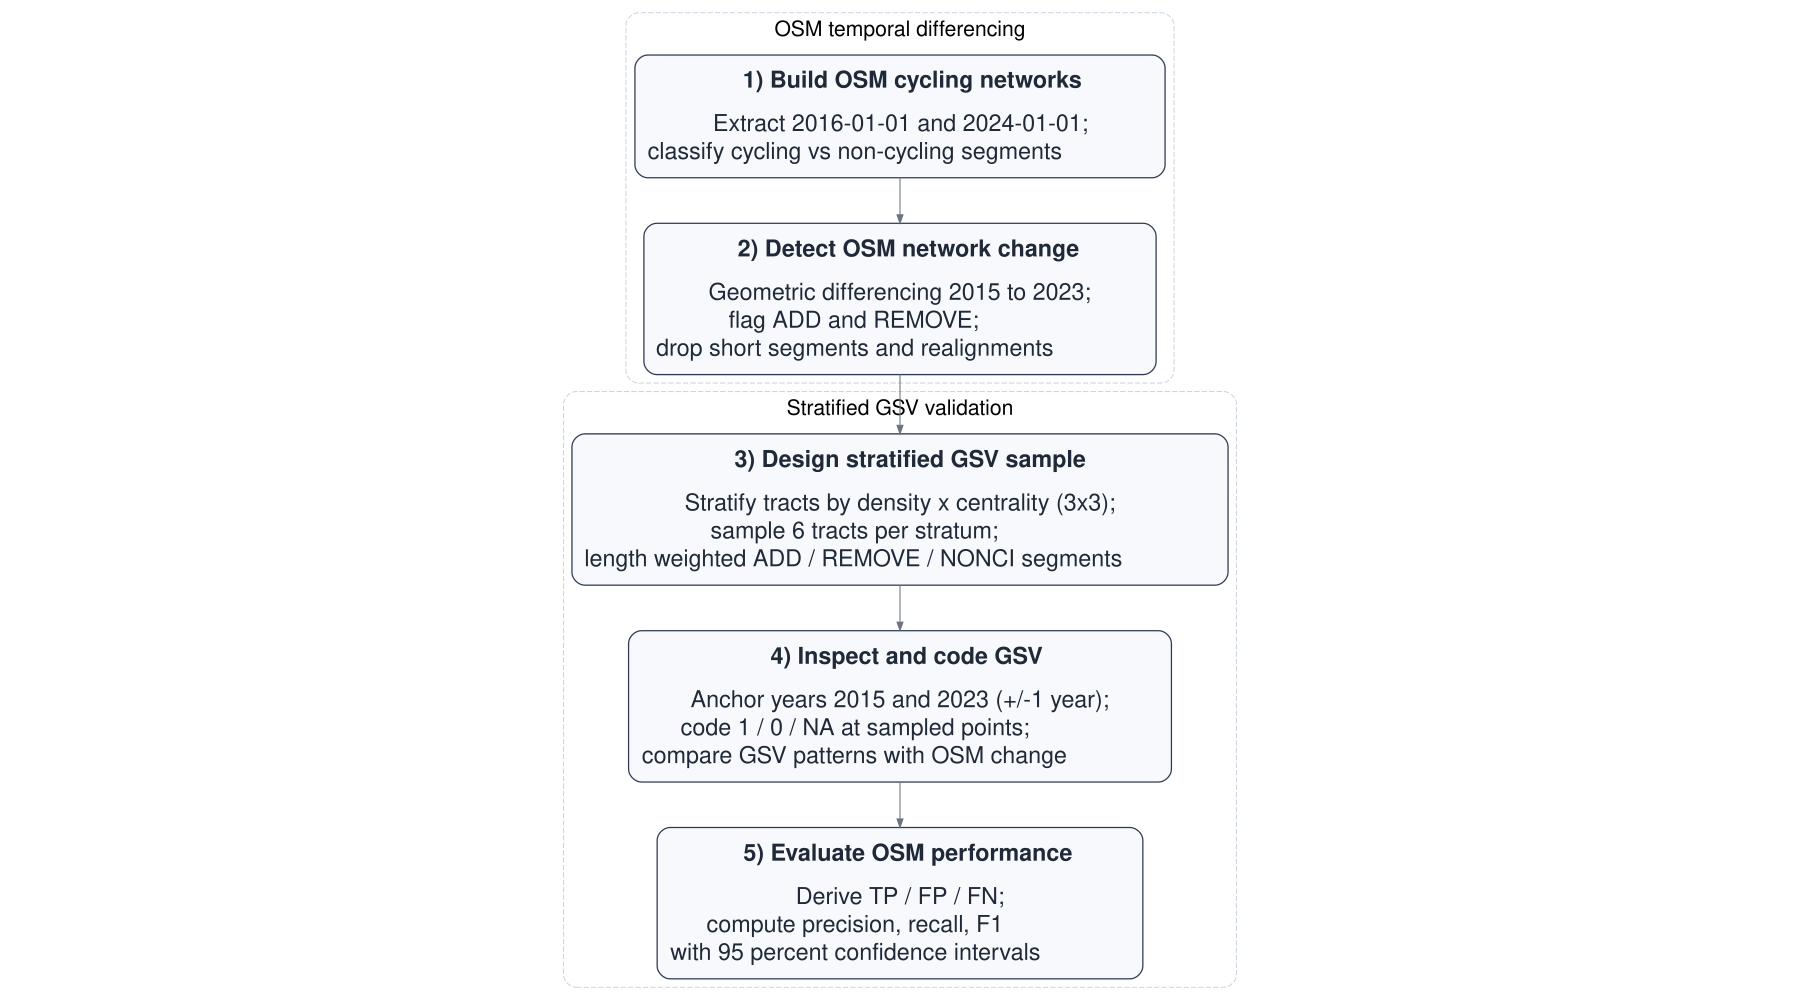
\includegraphics[width=1\linewidth,height=\textheight,keepaspectratio]{figs/osm_gsv_flowchart.png}

\caption{\label{fig-workflow}Workflow for detecting and validating
OSM-based cycling-infrastructure change, 2015--2023}

\end{figure}%

\subparagraph{OSM temporal
differencing}\label{osm-temporal-differencing}

Baseline and follow-up cycling networks were built from OSM extracts
dated 1 January 2016 and 1 January 2024 (approximating 2015 and 2023).
Road segments tagged as cycleways or otherwise designated for bicycle
use were classified as cycling infrastructure; all other urban segments
were treated as non-cycling.

After cleaning and projection, the two cycling network layers were
compared geometrically to identify added segments (present in 2023 only)
and removed segments (present in 2015 only). Small positional
realignments, where added and removed segments lay very close together,
were excluded so that minor mapping adjustments were not misclassified
as physical change.

\subparagraph{Stratified GSV
validation}\label{stratified-gsv-validation}

To validate these OSM-detected changes, we used a stratified sample of
Barcelona's 1,063 census tracts. Tracts were cross-classified by
population density and centrality into nine strata, from which six
tracts per stratum were randomly selected (54 in total). Within each
tract, up to two added, two removed, and one non-cycling segment were
sampled, with selection weighted by length. The midpoint of each sampled
segment served as the validation point and was linked to the nearest
available GSV panorama.

Each validation point was then assessed by two trained coders using GSV
panoramas for 2015 (baseline) and 2023 (follow-up). When imagery for the
target year was unavailable or obscured, the closest available years
were used (2024 and 2022 for follow-up; 2014 and 2016 for baseline).
Coders assigned 1 if cycling infrastructure was visible, 0 if absent,
and NA if indeterminate. Agreement was high: in 91 of 95 usable cases
(95.8 \%) both coders assigned the same code; disagreements were
resolved by consensus. Based on these observations, OSM-detected
additions were classed as True Positives (TP) when GSV showed a 0 to 1
pattern and as False Positives (FP) otherwise; removals were treated
analogously using 1 to 0 patterns, and non-cycling segments were used to
identify False Negatives (FN). Examples of TP additions and removals are
shown in Figure~\ref{fig-gsv-examples}.

\begin{figure}

\hfill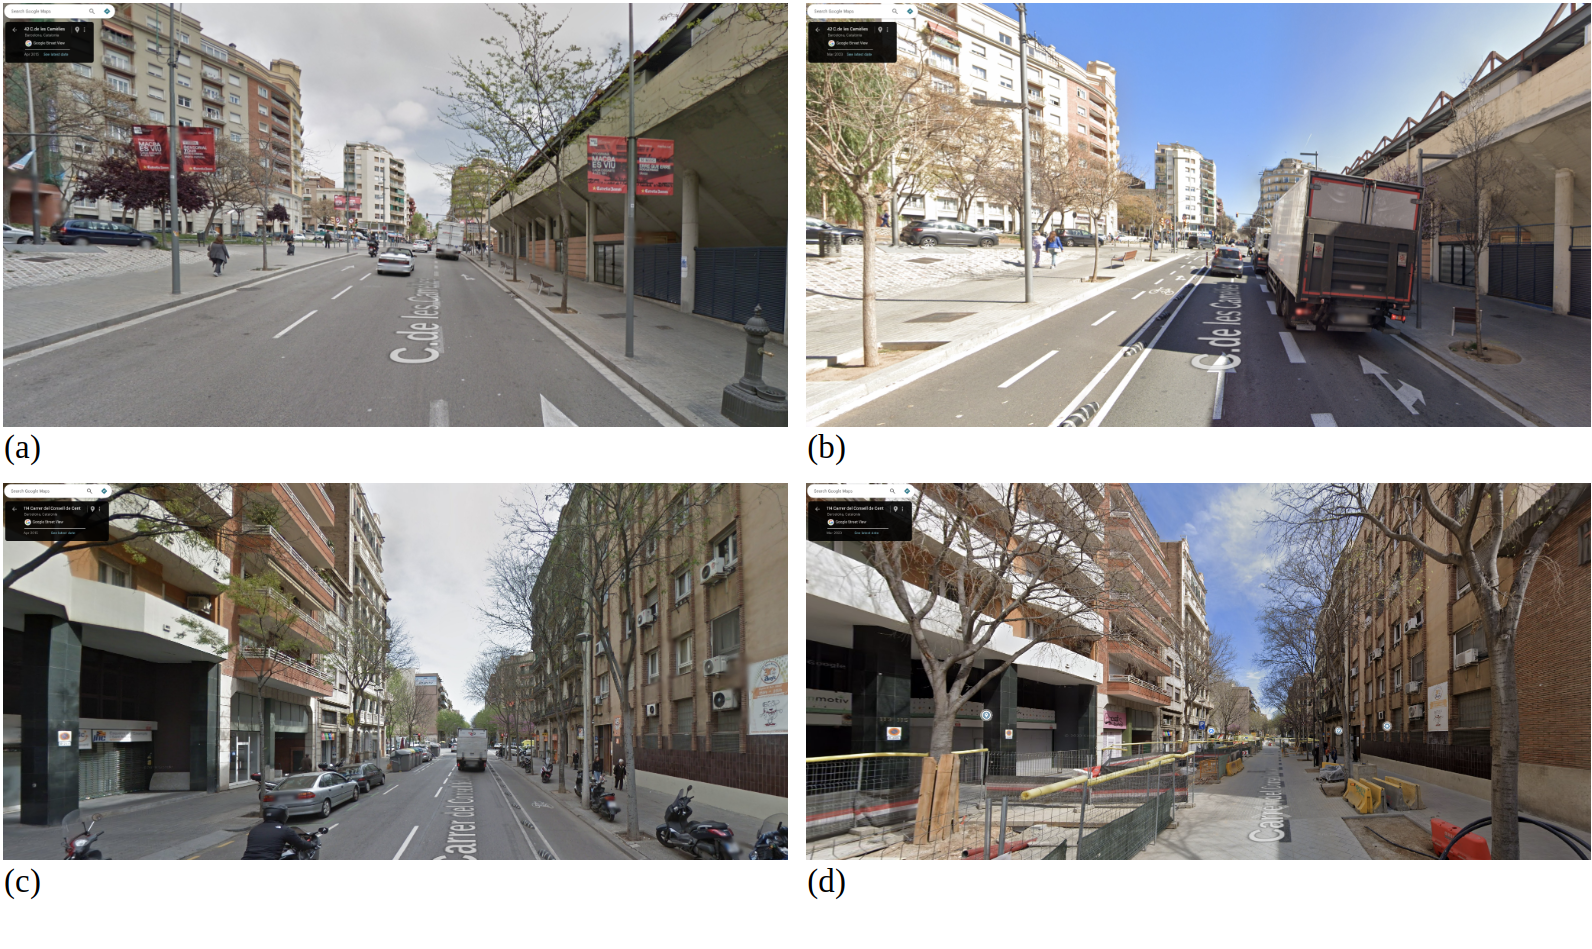
\includegraphics[width=1\linewidth,height=\textheight,keepaspectratio]{figs/fig-gsv-examples.png}

\caption{\label{fig-gsv-examples}Examples of True Positive changes
observed during GSV validation: (a) 2015 baseline with no cycling
infrastructure; (b) 2023 follow-up showing a new segregated track (0→1);
(c) 2015 baseline with a cycle track; (d) 2023 follow-up showing its
removal during a street redesign (1→0).}

\end{figure}%

Validation accuracy was then assessed using standard metrics. Precision
(TP/(TP+FP)) captures the share of OSM-detected changes that were real.
Recall (TP/(TP+FN)) captures the share of real changes correctly
detected by OSM. The F1 score is the harmonic mean of precision and
recall. Ninety-five per cent Wilson confidence intervals (CI) were
computed for each measure.

\subsection{Results and discussion}\label{results-and-discussion}

Between 2015 and 2023, the OSM-derived cycling network in Barcelona
increased from 153.6 to 288.4 km, representing an 88 \% expansion
(Figure~\ref{fig-map}). Geometric differencing indicated 156.0 km of
added and 24.8 km of removed infrastructure, corresponding to a net gain
of about 131 km. The small gap between this estimate and the change in
totals (--3.7 km) suggests good internal consistency. Additions were
concentrated in dense and central tracts, particularly high-density
areas close to the city core, which together accounted for roughly 58 \%
of the new network length. Removals were much less common and tended to
occur in intermediate-density areas.

\begin{figure}

\centering{

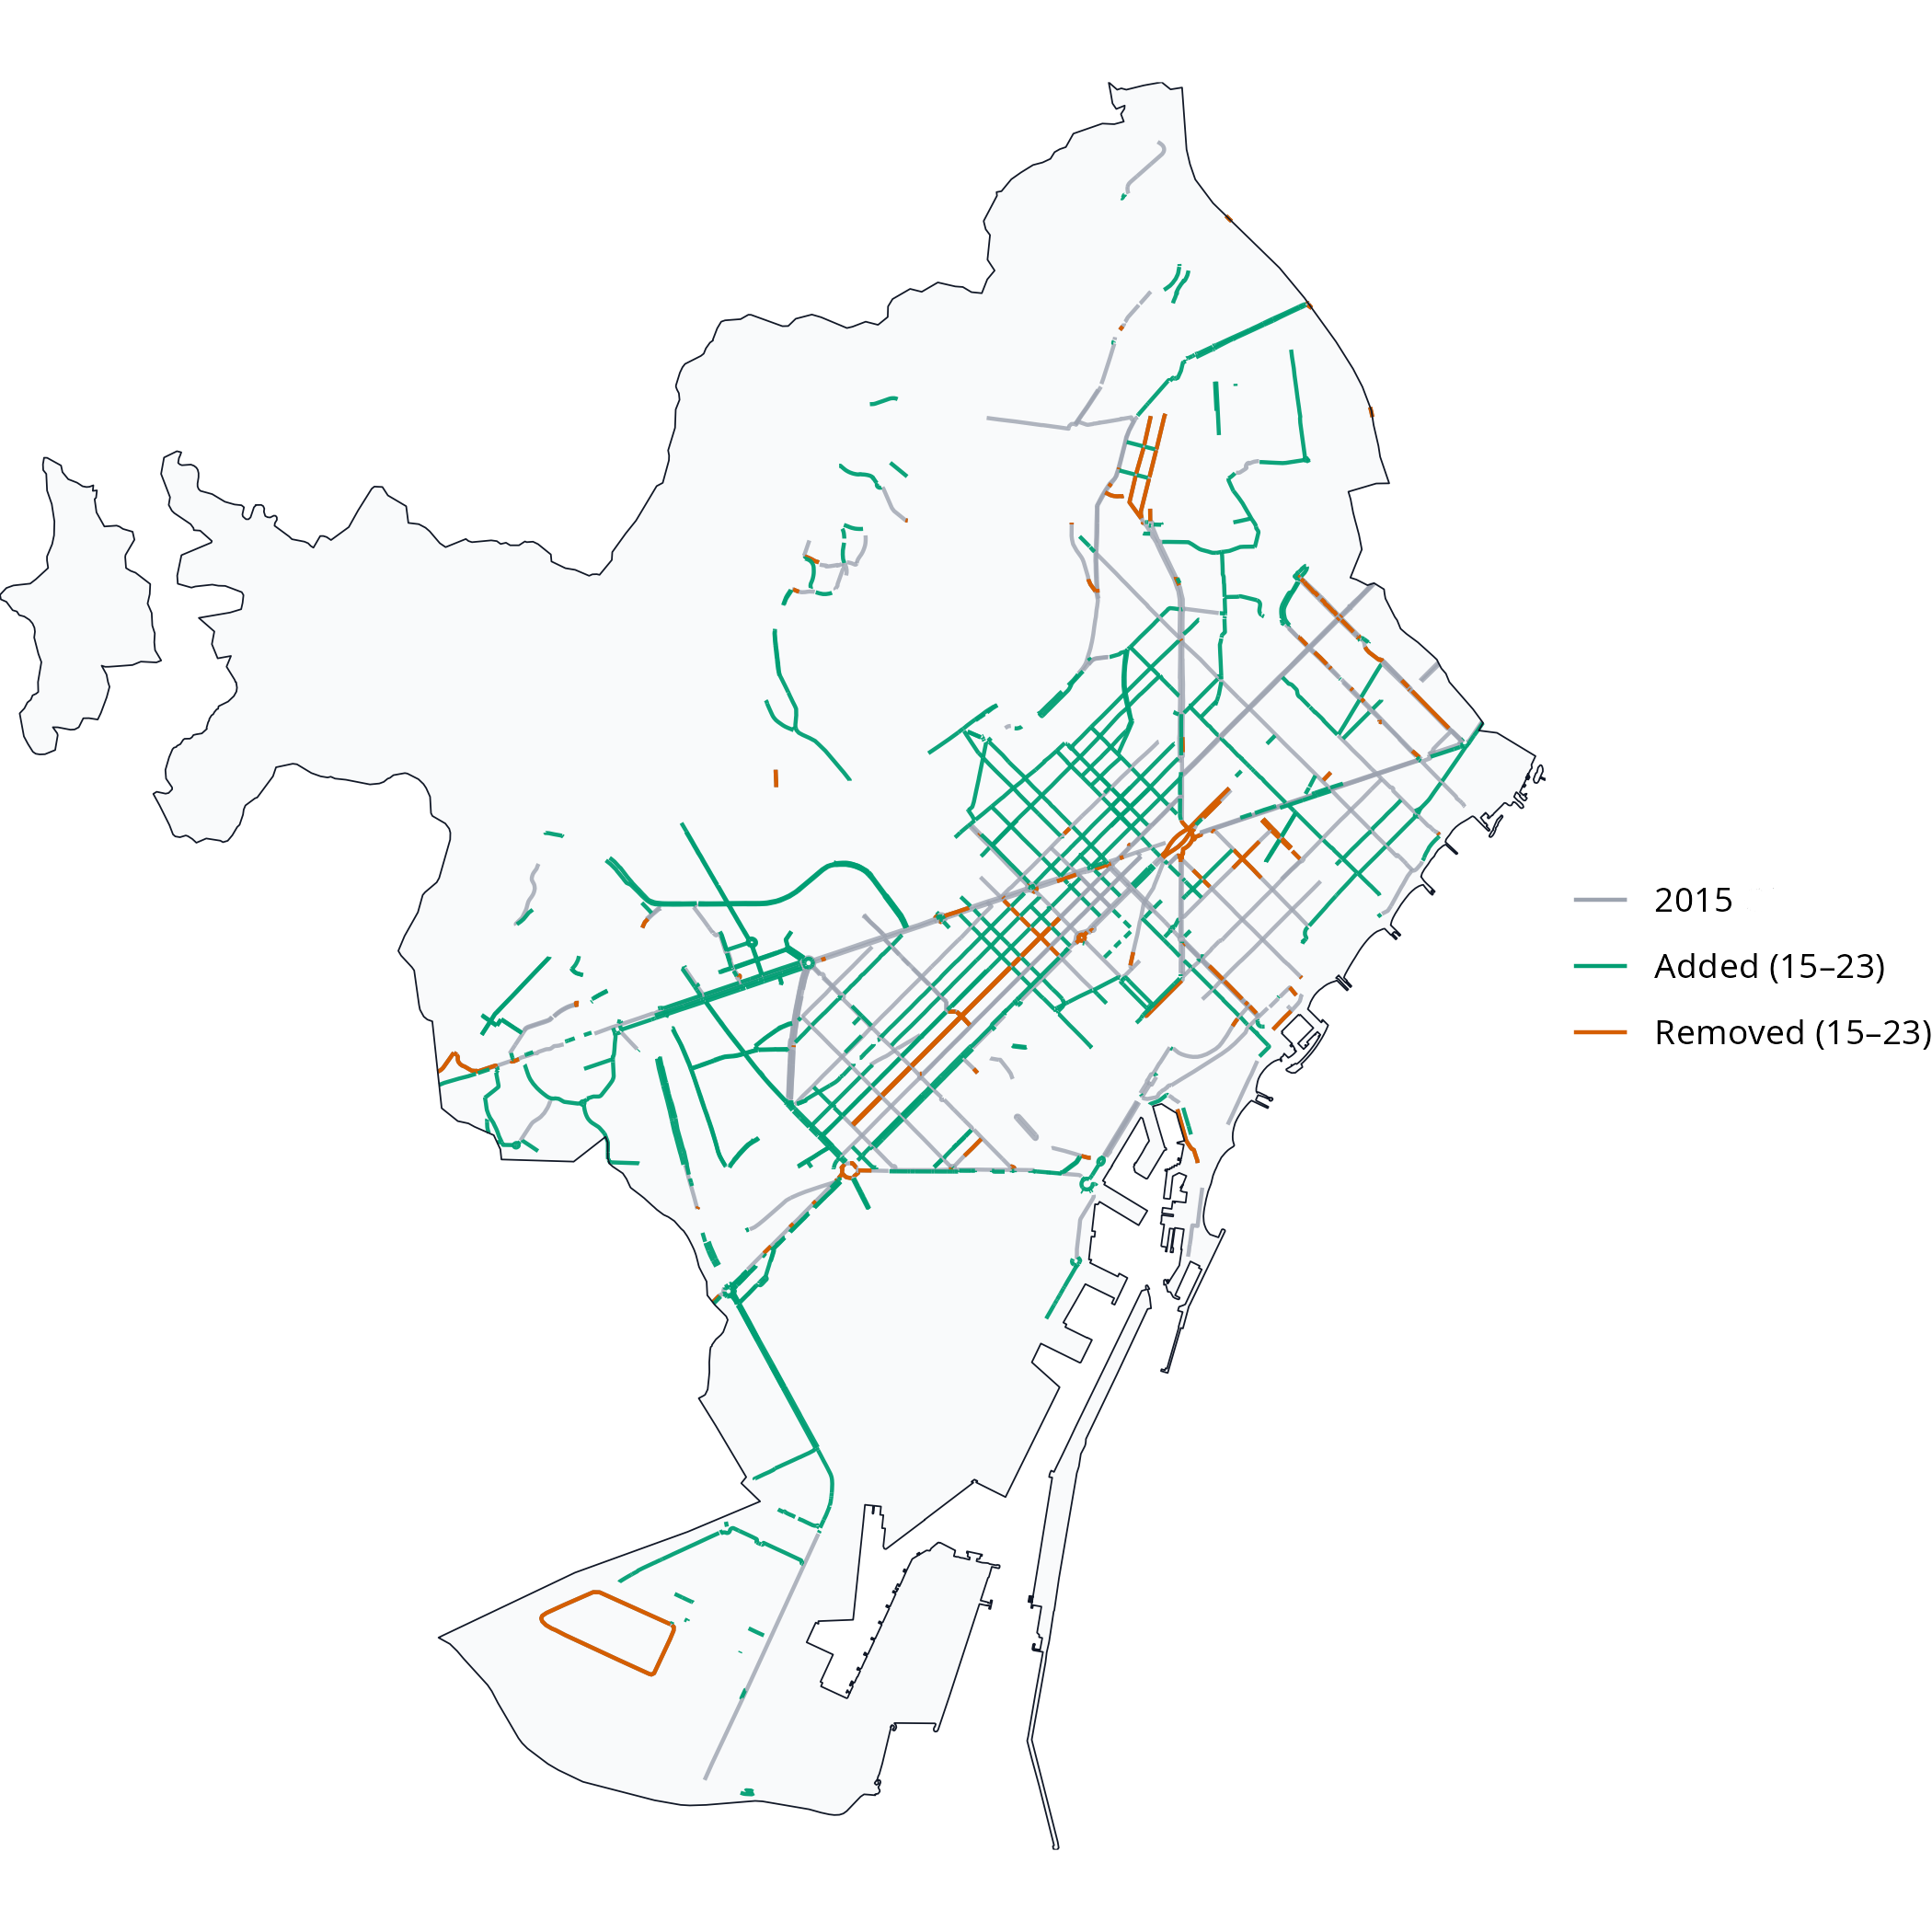
\includegraphics[width=1\linewidth,height=\textheight,keepaspectratio]{figs/infra_change_static2.png}

}

\caption{\label{fig-map}OSM-detected cycling-infrastructure changes in
Barcelona, 2015--2023.}

\end{figure}%

Of the 105 sampled sites, 95 (90 \%) provided usable GSV panoramas,
comprising 44 OSM-detected additions, 7 removals, and 44 non-cycling
controls. Table~\ref{tbl-validation} summarises the validation outcomes.

\begin{longtable}[]{@{}
  >{\raggedright\arraybackslash}p{(\linewidth - 14\tabcolsep) * \real{0.1029}}
  >{\raggedleft\arraybackslash}p{(\linewidth - 14\tabcolsep) * \real{0.1618}}
  >{\raggedleft\arraybackslash}p{(\linewidth - 14\tabcolsep) * \real{0.0441}}
  >{\raggedleft\arraybackslash}p{(\linewidth - 14\tabcolsep) * \real{0.0441}}
  >{\raggedleft\arraybackslash}p{(\linewidth - 14\tabcolsep) * \real{0.0441}}
  >{\raggedleft\arraybackslash}p{(\linewidth - 14\tabcolsep) * \real{0.2794}}
  >{\raggedleft\arraybackslash}p{(\linewidth - 14\tabcolsep) * \real{0.2500}}
  >{\raggedleft\arraybackslash}p{(\linewidth - 14\tabcolsep) * \real{0.0735}}@{}}

\caption{\label{tbl-validation}Validation metrics for OSM inferred
cycling-infrastructure changes (2015--2023). ``ADD'' refers to added
segments (present in 2023 but not in 2015); ``REMOVE'' refers to removed
segments (present in 2015 but not in 2023); ``Pooled'' combines both
change types. ``n (usable)'' is the number of sampled segments with
codable GSV panoramas for both years.}

\tabularnewline

\toprule\noalign{}
\begin{minipage}[b]{\linewidth}\raggedright
Class
\end{minipage} & \begin{minipage}[b]{\linewidth}\raggedleft
n (usable)
\end{minipage} & \begin{minipage}[b]{\linewidth}\raggedleft
TP
\end{minipage} & \begin{minipage}[b]{\linewidth}\raggedleft
FP
\end{minipage} & \begin{minipage}[b]{\linewidth}\raggedleft
FN
\end{minipage} & \begin{minipage}[b]{\linewidth}\raggedleft
Precision (95\% CI)
\end{minipage} & \begin{minipage}[b]{\linewidth}\raggedleft
Recall (95\% CI)
\end{minipage} & \begin{minipage}[b]{\linewidth}\raggedleft
F1
\end{minipage} \\
\midrule\noalign{}
\endhead
\bottomrule\noalign{}
\endlastfoot
ADD & 44 & 34 & 10 & 0 & 0.77 {[}0.63-0.87{]} & 1.00 {[}0.90-1.00{]} &
0.87 \\
REMOVE & 7 & 2 & 5 & 0 & 0.29 {[}0.08-0.64{]} & 1.00 {[}0.34-1.00{]} &
0.44 \\
Pooled & 51 & 36 & 15 & 0 & 0.71 {[}0.57-0.81{]} & 1.00 {[}0.90-1.00{]}
& 0.83 \\

\end{longtable}

Results show that OSM captures all observed additions (recall = 1.00, 95
\% CI {[}0.90--1.00{]}) but also includes some FP (precision \(\approx\)
0.77). For removals, recall was likewise 1.00 but with a wide CI due to
the small sample size, while precision drops sharply to around 0.29,
meaning that most apparent deletions do not correspond to true
infrastructure loss. Overall precision across all changes is 0.71 with
an F1 of 0.83.

Together, these results suggest that OSM is a strong proxy for additions
but a weaker one for removals. Although all real changes were captured,
OSM tended to flag more additions and removals than were visible in GSV.
Because the volume of apparent additions greatly exceeded that of
removals, this imbalance likely produces a slight overestimation of net
network growth when using raw OSM differencing.

A simple calibration using the observed precision values (0.77 for
additions, 0.29 for removals) can adjust OSM-based estimates of change,
reducing bias in net growth calculations. As validation was stratified
by density and centrality, calibration factors can be adapted to
specific urban contexts.

Methodologically, the study demonstrates a transparent, open-source
framework for assessing the temporal reliability of OSM data on cycling
infrastructure. The workflow, combining historical differencing,
stratified sampling, and visual inspection, is reproducible in any city
with sufficient Street View coverage. It underpins the ATRAPA Built
Environment Transformations Dataset, which will extend this validation
approach to other European cities including Milan, Ljubljana, Warsaw,
Utrecht, Malmö, and Paris.

Theoretically, this work supports the view of OSM as a dynamic
socio-technical system rather than a static dataset. Temporal variation
in OSM reflects both genuine infrastructure evolution and the rhythms of
community mapping activity. By distinguishing true from apparent edits,
the approach contributes to a broader framework for assessing the
temporal validity of VGI -- an essential step for longitudinal research
in transport, health, and environmental studies.

Several limitations should be acknowledged. True removals were few,
producing wide confidence intervals for that category. GSV imagery dates
vary within each anchor year, occasionally creating minor temporal
mismatches. Although inter-rater agreement was high, subtle interpretive
differences -- for example, in deciding whether a feature should count
as cycling infrastructure or not -- remain possible. Finally,
Barcelona's large and active mapping community likely ensures relatively
high data quality; replication in less-mapped cities will be required to
test generalisability.

\subsection{Conclusions and
implications}\label{conclusions-and-implications}

This Barcelona pilot demonstrates that OSM can reliably detect additions
to cycling infrastructure but struggles to capture removals. Overall,
OSM slightly overstates network growth. Despite these limitations, OSM
remains a valuable, low-cost resource for longitudinal analysis of
cycling infrastructure when accompanied by empirical calibration.

The study introduces a transparent validation framework that combines
OSM historical data, stratified sampling, and GSV-based inspection to
generate quantitative precision and recall metrics. These can be used to
correct OSM-derived measures of change and to support comparisons within
the ATRAPA framework. More broadly, the findings strengthen confidence
in using VGI for temporal urban analysis while highlighting the need to
understand the social and temporal dynamics behind its production.

\subsection*{Acknowledgements}\label{acknowledgements}
\addcontentsline{toc}{subsection}{Acknowledgements}

This research forms part of the ATRAPA project and is funded by the
European Research Council (grant 101117700). We also thank Víctor
González Parra for his collaboration as second coder during the Google
Street View validation and the OpenStreetMap community for their
contributions.

\subsection*{References}\label{references}
\addcontentsline{toc}{subsection}{References}

\phantomsection\label{refs}
\begin{CSLReferences}{1}{0}
\bibitem[\citeproctext]{ref-barron_comprehensive_2014}
Barron, C., Neis, P., Zipf, A., 2014. A {Comprehensive} {Framework} for
{Intrinsic} {OpenStreetMap} {Quality} {Analysis}. Transactions in GIS
18, 877--895. \url{https://doi.org/10.1111/tgis.12073}

\bibitem[\citeproctext]{ref-buehler_cycling_2021}
Buehler, R., Pucher, J. (Eds.), 2021. Cycling for sustainable cities,
Urban and {Industrial} {Environments}. MIT Press, Cambridge.

\bibitem[\citeproctext]{ref-ferster_using_2020}
Ferster, C., Fischer, J., Manaugh, K., Nelson, T., Winters, M., 2020.
Using {OpenStreetMap} to inventory bicycle infrastructure: {A}
comparison with open data from cities. International Journal of
Sustainable Transportation 14, 64--73.
\url{https://doi.org/10.1080/15568318.2018.1519746}

\bibitem[\citeproctext]{ref-gemott_research_group_atrapa_2025}
GEMOTT Research Group, 2025.
\href{https://webs.uab.cat/atrapa/}{{ATRAPA} -- {The} {Active} {Travel}
{Backlash} {Paradox}}.

\bibitem[\citeproctext]{ref-goodchild_citizens_2007}
Goodchild, M.F., 2007. Citizens as sensors: The world of volunteered
geography. GeoJournal 69, 211--221.
\url{https://doi.org/10.1007/s10708-007-9111-y}

\bibitem[\citeproctext]{ref-szell_growing_2022}
Szell, M., Mimar, S., Perlman, T., Ghoshal, G., Sinatra, R., 2022.
Growing urban bicycle networks. Scientific Reports 12, 6765.
\url{https://doi.org/10.1038/s41598-022-10783-y}

\bibitem[\citeproctext]{ref-viero_how_2025}
Vierø, A.R., Vybornova, A., Szell, M., 2025. How {Good} {Is} {Open}
{Bicycle} {Network} {Data}? {A} {Countrywide} {Case} {Study} of
{Denmark}. Geographical Analysis 57, 52--87.
\url{https://doi.org/10.1111/gean.12400}

\end{CSLReferences}




\end{document}
